% Générée par docs/rhm/figures.mjs à partir de src/content/math-map.json (2026-09-26) — ne pas éditer à la main.
\begin{figure}[htbp]\centering
\definecolor{dat0}{RGB}{151,175,225}
\definecolor{dat1}{RGB}{107,138,208}
\definecolor{dat2}{RGB}{74,107,189}
\definecolor{dat3}{RGB}{46,68,127}
\definecolor{dat4}{RGB}{34,49,84}
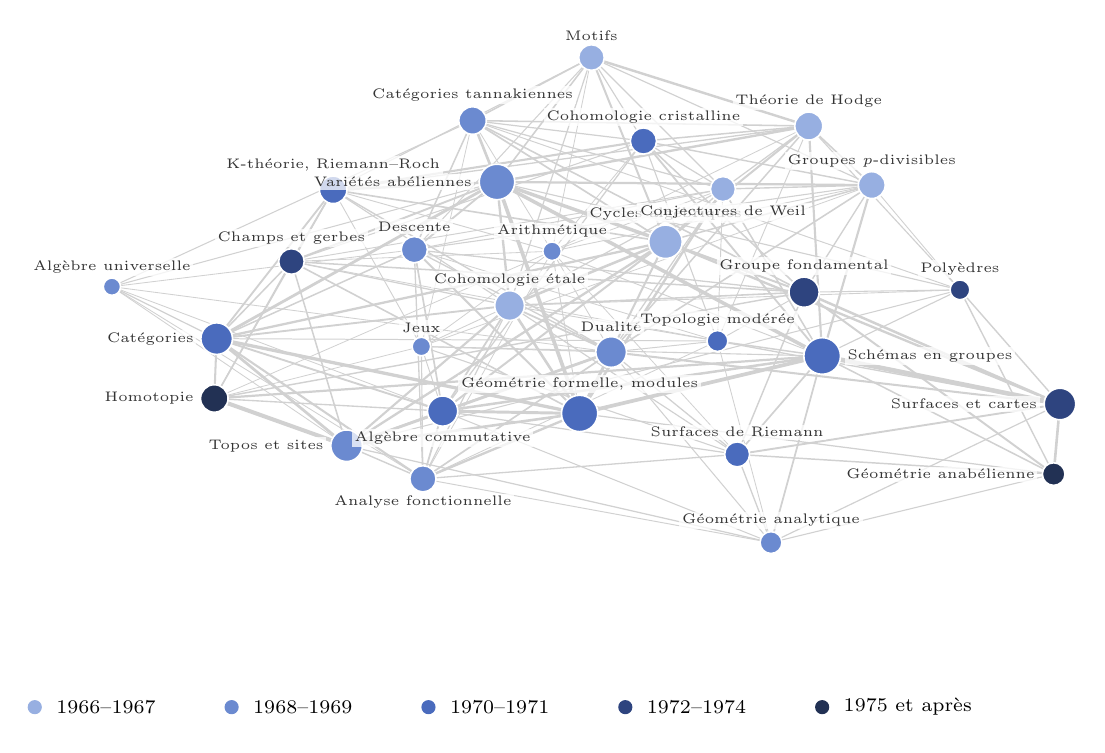
\begin{tikzpicture}
\draw[black!18,line width=0.66pt] (5.18,3.21) -- (7.32,3.96);
\draw[black!18,line width=0.65pt] (5.18,3.21) -- (4.93,2.35);
\draw[black!18,line width=0.35pt] (5.18,3.21) -- (4.91,4.03);
\draw[black!18,line width=0.90pt] (5.18,3.21) -- (10.00,3.91);
\draw[black!18,line width=0.45pt] (5.18,3.21) -- (8.92,2.66);
\draw[black!18,line width=0.65pt] (5.18,3.21) -- (6.03,4.55);
\draw[black!18,line width=0.61pt] (7.32,3.96) -- (4.93,2.35);
\draw[black!18,line width=0.36pt] (7.32,3.96) -- (4.91,4.03);
\draw[black!18,line width=0.46pt] (7.32,3.96) -- (8.92,2.66);
\draw[black!18,line width=0.64pt] (7.32,3.96) -- (6.03,4.55);
\draw[black!18,line width=0.40pt] (4.93,2.35) -- (4.91,4.03);
\draw[black!18,line width=0.47pt] (4.93,2.35) -- (8.92,2.66);
\draw[black!18,line width=0.46pt] (4.93,2.35) -- (6.03,4.55);
\draw[black!18,line width=0.40pt] (4.91,4.03) -- (10.00,3.91);
\draw[black!18,line width=0.40pt] (4.91,4.03) -- (8.92,2.66);
\draw[black!18,line width=0.32pt] (4.91,4.03) -- (6.03,4.55);
\draw[black!18,line width=0.61pt] (10.00,3.91) -- (8.92,2.66);
\draw[black!18,line width=1.25pt] (5.87,6.12) -- (8.01,5.36);
\draw[black!18,line width=1.01pt] (5.87,6.12) -- (2.31,4.13);
\draw[black!18,line width=0.86pt] (5.87,6.12) -- (3.79,6.02);
\draw[black!18,line width=0.83pt] (8.01,5.36) -- (2.31,4.13);
\draw[black!18,line width=0.85pt] (8.01,5.36) -- (13.02,3.30);
\draw[black!18,line width=0.71pt] (8.01,5.36) -- (9.77,4.72);
\draw[black!18,line width=0.59pt] (8.01,5.36) -- (3.79,6.02);
\draw[black!18,line width=0.84pt] (8.01,5.36) -- (3.96,2.77);
\draw[black!18,line width=0.67pt] (2.31,4.13) -- (3.79,6.02);
\draw[black!18,line width=0.99pt] (2.31,4.13) -- (3.96,2.77);
\draw[black!18,line width=0.90pt] (13.02,3.30) -- (9.77,4.72);
\draw[black!18,line width=0.69pt] (13.02,3.30) -- (8.92,2.66);
\draw[black!18,line width=0.52pt] (9.77,4.72) -- (8.92,2.66);
\draw[black!18,line width=0.42pt] (3.79,6.02) -- (8.92,2.66);
\draw[black!18,line width=0.65pt] (5.87,6.12) -- (4.82,5.26);
\draw[black!18,line width=1.33pt] (5.87,6.12) -- (6.92,3.18);
\draw[black!18,line width=1.29pt] (5.87,6.12) -- (10.00,3.91);
\draw[black!18,line width=0.86pt] (5.87,6.12) -- (9.83,6.83);
\draw[black!18,line width=0.57pt] (5.87,6.12) -- (7.07,7.70);
\draw[black!18,line width=0.70pt] (5.87,6.12) -- (3.26,5.11);
\draw[black!18,line width=0.96pt] (5.87,6.12) -- (5.56,6.90);
\draw[black!18,line width=0.81pt] (5.87,6.12) -- (10.63,6.08);
\draw[black!18,line width=0.74pt] (8.01,5.36) -- (9.83,6.83);
\draw[black!18,line width=0.72pt] (8.01,5.36) -- (7.07,7.70);
\draw[black!18,line width=0.61pt] (8.01,5.36) -- (5.56,6.90);
\draw[black!18,line width=0.49pt] (8.01,5.36) -- (8.74,6.03);
\draw[black!18,line width=0.54pt] (8.01,5.36) -- (10.63,6.08);
\draw[black!18,line width=1.65pt] (13.02,3.30) -- (10.00,3.91);
\draw[black!18,line width=0.56pt] (7.73,6.64) -- (9.77,4.72);
\draw[black!18,line width=0.66pt] (7.73,6.64) -- (10.00,3.91);
\draw[black!18,line width=0.54pt] (7.73,6.64) -- (9.83,6.83);
\draw[black!18,line width=0.76pt] (7.73,6.64) -- (3.79,6.02);
\draw[black!18,line width=0.42pt] (7.73,6.64) -- (7.07,7.70);
\draw[black!18,line width=0.30pt] (7.73,6.64) -- (6.57,5.24);
\draw[black!18,line width=0.38pt] (7.73,6.64) -- (3.26,5.11);
\draw[black!18,line width=0.44pt] (7.73,6.64) -- (5.56,6.90);
\draw[black!18,line width=0.44pt] (7.73,6.64) -- (8.74,6.03);
\draw[black!18,line width=0.52pt] (7.73,6.64) -- (10.63,6.08);
\draw[black!18,line width=0.73pt] (4.82,5.26) -- (6.92,3.18);
\draw[black!18,line width=0.47pt] (4.82,5.26) -- (9.77,4.72);
\draw[black!18,line width=0.38pt] (4.82,5.26) -- (7.07,7.70);
\draw[black!18,line width=0.55pt] (4.82,5.26) -- (5.56,6.90);
\draw[black!18,line width=0.37pt] (4.82,5.26) -- (8.74,6.03);
\draw[black!18,line width=0.40pt] (4.82,5.26) -- (10.63,6.08);
\draw[black!18,line width=1.34pt] (6.92,3.18) -- (10.00,3.91);
\draw[black!18,line width=0.34pt] (6.92,3.18) -- (6.57,5.24);
\draw[black!18,line width=0.58pt] (6.92,3.18) -- (3.26,5.11);
\draw[black!18,line width=0.86pt] (6.92,3.18) -- (8.74,6.03);
\draw[black!18,line width=0.55pt] (9.77,4.72) -- (3.26,5.11);
\draw[black!18,line width=0.57pt] (9.77,4.72) -- (5.56,6.90);
\draw[black!18,line width=0.49pt] (9.77,4.72) -- (10.63,6.08);
\draw[black!18,line width=0.77pt] (10.00,3.91) -- (9.83,6.83);
\draw[black!18,line width=0.34pt] (10.00,3.91) -- (6.57,5.24);
\draw[black!18,line width=0.56pt] (10.00,3.91) -- (8.74,6.03);
\draw[black!18,line width=0.78pt] (10.00,3.91) -- (10.63,6.08);
\draw[black!18,line width=0.47pt] (9.83,6.83) -- (3.79,6.02);
\draw[black!18,line width=0.88pt] (9.83,6.83) -- (7.07,7.70);
\draw[black!18,line width=0.30pt] (9.83,6.83) -- (6.57,5.24);
\draw[black!18,line width=0.56pt] (9.83,6.83) -- (5.56,6.90);
\draw[black!18,line width=0.46pt] (9.83,6.83) -- (8.74,6.03);
\draw[black!18,line width=0.58pt] (9.83,6.83) -- (10.63,6.08);
\draw[black!18,line width=0.40pt] (3.79,6.02) -- (7.07,7.70);
\draw[black!18,line width=0.34pt] (3.79,6.02) -- (6.57,5.24);
\draw[black!18,line width=0.61pt] (3.79,6.02) -- (3.26,5.11);
\draw[black!18,line width=0.30pt] (7.07,7.70) -- (6.57,5.24);
\draw[black!18,line width=0.55pt] (7.07,7.70) -- (5.56,6.90);
\draw[black!18,line width=0.47pt] (7.07,7.70) -- (8.74,6.03);
\draw[black!18,line width=0.42pt] (7.07,7.70) -- (10.63,6.08);
\draw[black!18,line width=0.30pt] (6.57,5.24) -- (3.26,5.11);
\draw[black!18,line width=0.30pt] (6.57,5.24) -- (5.56,6.90);
\draw[black!18,line width=0.30pt] (6.57,5.24) -- (8.74,6.03);
\draw[black!18,line width=0.32pt] (6.57,5.24) -- (10.63,6.08);
\draw[black!18,line width=0.35pt] (3.26,5.11) -- (8.74,6.03);
\draw[black!18,line width=0.45pt] (5.56,6.90) -- (8.74,6.03);
\draw[black!18,line width=0.50pt] (8.74,6.03) -- (10.63,6.08);
\draw[black!18,line width=0.73pt] (8.01,5.36) -- (7.32,3.96);
\draw[black!18,line width=0.92pt] (8.01,5.36) -- (6.03,4.55);
\draw[black!18,line width=0.45pt] (7.32,3.96) -- (8.74,6.03);
\draw[black!18,line width=0.44pt] (7.07,7.70) -- (6.03,4.55);
\draw[black!18,line width=0.43pt] (8.74,6.03) -- (6.03,4.55);
\draw[black!18,line width=0.86pt] (5.87,6.12) -- (6.03,4.55);
\draw[black!18,line width=0.72pt] (8.01,5.36) -- (5.18,3.21);
\draw[black!18,line width=0.68pt] (2.31,4.13) -- (5.18,3.21);
\draw[black!18,line width=0.54pt] (2.31,4.13) -- (4.82,5.26);
\draw[black!18,line width=1.19pt] (2.31,4.13) -- (6.92,3.18);
\draw[black!18,line width=0.75pt] (2.31,4.13) -- (4.93,2.35);
\draw[black!18,line width=0.55pt] (2.31,4.13) -- (3.26,5.11);
\draw[black!18,line width=0.68pt] (2.31,4.13) -- (6.03,4.55);
\draw[black!18,line width=0.61pt] (5.18,3.21) -- (4.82,5.26);
\draw[black!18,line width=1.07pt] (5.18,3.21) -- (6.92,3.18);
\draw[black!18,line width=0.73pt] (5.18,3.21) -- (3.96,2.77);
\draw[black!18,line width=0.48pt] (4.82,5.26) -- (7.32,3.96);
\draw[black!18,line width=0.48pt] (4.82,5.26) -- (4.93,2.35);
\draw[black!18,line width=1.05pt] (7.32,3.96) -- (6.92,3.18);
\draw[black!18,line width=0.54pt] (7.32,3.96) -- (9.83,6.83);
\draw[black!18,line width=0.52pt] (7.32,3.96) -- (3.79,6.02);
\draw[black!18,line width=1.02pt] (7.32,3.96) -- (3.96,2.77);
\draw[black!18,line width=0.57pt] (7.32,3.96) -- (10.63,6.08);
\draw[black!18,line width=0.85pt] (6.92,3.18) -- (4.93,2.35);
\draw[black!18,line width=0.94pt] (6.92,3.18) -- (3.96,2.77);
\draw[black!18,line width=0.95pt] (6.92,3.18) -- (6.03,4.55);
\draw[black!18,line width=0.51pt] (4.93,2.35) -- (3.96,2.77);
\draw[black!18,line width=0.57pt] (9.77,4.72) -- (6.03,4.55);
\draw[black!18,line width=0.55pt] (3.26,5.11) -- (3.96,2.77);
\draw[black!18,line width=0.45pt] (3.26,5.11) -- (6.03,4.55);
\draw[black!18,line width=0.77pt] (3.96,2.77) -- (6.03,4.55);
\draw[black!18,line width=0.48pt] (13.02,3.30) -- (8.67,4.10);
\draw[black!18,line width=0.40pt] (7.73,6.64) -- (8.67,4.10);
\draw[black!18,line width=0.34pt] (9.77,4.72) -- (8.67,4.10);
\draw[black!18,line width=0.54pt] (10.00,3.91) -- (8.67,4.10);
\draw[black!18,line width=0.34pt] (9.83,6.83) -- (8.67,4.10);
\draw[black!18,line width=0.34pt] (8.67,4.10) -- (8.74,6.03);
\draw[black!18,line width=0.34pt] (8.67,4.10) -- (6.03,4.55);
\draw[black!18,line width=0.74pt] (13.02,3.30) -- (7.32,3.96);
\draw[black!18,line width=0.46pt] (5.18,3.21) -- (7.73,6.64);
\draw[black!18,line width=0.32pt] (7.32,3.96) -- (6.57,5.24);
\draw[black!18,line width=0.38pt] (5.18,3.21) -- (9.35,1.54);
\draw[black!18,line width=0.38pt] (9.35,1.54) -- (7.32,3.96);
\draw[black!18,line width=0.35pt] (9.35,1.54) -- (4.93,2.35);
\draw[black!18,line width=0.48pt] (9.35,1.54) -- (8.92,2.66);
\draw[black!18,line width=0.36pt] (2.31,4.13) -- (8.67,4.10);
\draw[black!18,line width=0.31pt] (9.35,1.54) -- (8.67,4.10);
\draw[black!18,line width=0.31pt] (4.82,5.26) -- (8.67,4.10);
\draw[black!18,line width=0.36pt] (7.32,3.96) -- (8.67,4.10);
\draw[black!18,line width=0.31pt] (4.93,2.35) -- (8.67,4.10);
\draw[black!18,line width=0.52pt] (9.77,4.72) -- (2.28,3.37);
\draw[black!18,line width=0.80pt] (10.00,3.91) -- (2.28,3.37);
\draw[black!18,line width=0.49pt] (2.28,3.37) -- (3.79,6.02);
\draw[black!18,line width=0.56pt] (2.28,3.37) -- (3.26,5.11);
\draw[black!18,line width=1.46pt] (2.28,3.37) -- (3.96,2.77);
\draw[black!18,line width=0.49pt] (5.18,3.21) -- (2.28,3.37);
\draw[black!18,line width=0.41pt] (5.87,6.12) -- (11.75,4.75);
\draw[black!18,line width=0.41pt] (10.00,3.91) -- (11.75,4.75);
\draw[black!18,line width=0.41pt] (9.83,6.83) -- (11.75,4.75);
\draw[black!18,line width=0.35pt] (11.75,4.75) -- (5.56,6.90);
\draw[black!18,line width=0.32pt] (11.75,4.75) -- (10.63,6.08);
\draw[black!18,line width=0.32pt] (11.75,4.75) -- (6.03,4.55);
\draw[black!18,line width=0.63pt] (9.35,1.54) -- (10.00,3.91);
\draw[black!18,line width=0.45pt] (9.35,1.54) -- (3.96,2.77);
\draw[black!18,line width=0.94pt] (12.94,2.41) -- (13.02,3.30);
\draw[black!18,line width=0.40pt] (12.94,2.41) -- (9.35,1.54);
\draw[black!18,line width=0.45pt] (12.94,2.41) -- (6.92,3.18);
\draw[black!18,line width=0.71pt] (12.94,2.41) -- (9.77,4.72);
\draw[black!18,line width=0.55pt] (12.94,2.41) -- (10.00,3.91);
\draw[black!18,line width=0.53pt] (12.94,2.41) -- (8.92,2.66);
\draw[black!18,line width=0.43pt] (13.02,3.30) -- (9.35,1.54);
\draw[black!18,line width=0.33pt] (4.91,4.03) -- (3.79,6.02);
\draw[black!18,line width=0.29pt] (4.91,4.03) -- (5.56,6.90);
\draw[black!18,line width=0.51pt] (12.94,2.41) -- (11.75,4.75);
\draw[black!18,line width=0.51pt] (13.02,3.30) -- (11.75,4.75);
\draw[black!18,line width=0.38pt] (9.77,4.72) -- (11.75,4.75);
\draw[black!18,line width=0.74pt] (2.31,4.13) -- (2.28,3.37);
\draw[black!18,line width=0.29pt] (4.93,2.35) -- (6.57,5.24);
\draw[black!18,line width=0.29pt] (4.91,4.03) -- (2.28,3.37);
\draw[black!18,line width=0.29pt] (4.91,4.03) -- (6.57,5.24);
\draw[black!18,line width=0.29pt] (4.91,4.03) -- (10.63,6.08);
\draw[black!18,line width=0.29pt] (2.28,3.37) -- (6.57,5.24);
\draw[black!18,line width=0.29pt] (6.57,5.24) -- (8.92,2.66);
\draw[black!18,line width=0.31pt] (3.26,5.11) -- (8.67,4.10);
\draw[black!18,line width=0.38pt] (5.87,6.12) -- (0.98,4.79);
\draw[black!18,line width=0.44pt] (2.31,4.13) -- (0.98,4.79);
\draw[black!18,line width=0.38pt] (5.56,6.90) -- (0.98,4.79);
\draw[black!18,line width=0.31pt] (5.18,3.21) -- (0.98,4.79);
\draw[black!18,line width=0.31pt] (4.82,5.26) -- (0.98,4.79);
\draw[black!18,line width=0.31pt] (7.32,3.96) -- (0.98,4.79);
\draw[black!18,line width=0.31pt] (4.93,2.35) -- (0.98,4.79);
\draw[black!18,line width=0.31pt] (3.96,2.77) -- (0.98,4.79);
\draw[black!18,line width=0.38pt] (11.75,4.75) -- (3.96,2.77);
\fill[dat1,draw=white,line width=0.6pt] (3.96,2.77) circle (0.201);
\fill[dat3,draw=white,line width=0.6pt] (3.26,5.11) circle (0.163);
\fill[dat4,draw=white,line width=0.6pt] (2.28,3.37) circle (0.175);
\fill[dat2,draw=white,line width=0.6pt] (2.31,4.13) circle (0.201);
\fill[dat1,draw=white,line width=0.6pt] (5.56,6.90) circle (0.175);
\fill[dat0,draw=white,line width=0.6pt] (7.07,7.70) circle (0.163);
\fill[dat0,draw=white,line width=0.6pt] (8.01,5.36) circle (0.213);
\fill[dat0,draw=white,line width=0.6pt] (9.83,6.83) circle (0.178);
\fill[dat0,draw=white,line width=0.6pt] (8.74,6.03) circle (0.159);
\fill[dat0,draw=white,line width=0.6pt] (6.03,4.55) circle (0.189);
\fill[dat2,draw=white,line width=0.6pt] (7.73,6.64) circle (0.167);
\fill[dat0,draw=white,line width=0.6pt] (10.63,6.08) circle (0.171);
\fill[dat1,draw=white,line width=0.6pt] (5.87,6.12) circle (0.226);
\fill[dat2,draw=white,line width=0.6pt] (10.00,3.91) circle (0.233);
\fill[dat1,draw=white,line width=0.6pt] (4.82,5.26) circle (0.167);
\fill[dat3,draw=white,line width=0.6pt] (9.77,4.72) circle (0.192);
\fill[dat4,draw=white,line width=0.6pt] (12.94,2.41) circle (0.144);
\fill[dat1,draw=white,line width=0.6pt] (7.32,3.96) circle (0.195);
\fill[dat2,draw=white,line width=0.6pt] (3.79,6.02) circle (0.175);
\fill[dat2,draw=white,line width=0.6pt] (5.18,3.21) circle (0.192);
\fill[dat1,draw=white,line width=0.6pt] (4.93,2.35) circle (0.167);
\fill[dat3,draw=white,line width=0.6pt] (13.02,3.30) circle (0.201);
\fill[dat3,draw=white,line width=0.6pt] (11.75,4.75) circle (0.126);
\fill[dat2,draw=white,line width=0.6pt] (8.67,4.10) circle (0.133);
\fill[dat1,draw=white,line width=0.6pt] (6.57,5.24) circle (0.118);
\fill[dat1,draw=white,line width=0.6pt] (9.35,1.54) circle (0.139);
\fill[dat1,draw=white,line width=0.6pt] (0.98,4.79) circle (0.110);
\fill[dat2,draw=white,line width=0.6pt] (6.92,3.18) circle (0.231);
\fill[dat2,draw=white,line width=0.6pt] (8.92,2.66) circle (0.159);
\fill[dat1,draw=white,line width=0.6pt] (4.91,4.03) circle (0.118);
\node[font=\tiny,text=black!80,anchor=east,inner sep=1pt,fill=white,fill opacity=0.75,text opacity=1] at (3.71,2.77) {Topos et sites};
\node[font=\tiny,text=black!80,anchor=south,inner sep=1pt,fill=white,fill opacity=0.75,text opacity=1] at (3.26,5.29) {Champs et gerbes};
\node[font=\tiny,text=black!80,anchor=east,inner sep=1pt,fill=white,fill opacity=0.75,text opacity=1] at (2.06,3.37) {Homotopie};
\node[font=\tiny,text=black!80,anchor=east,inner sep=1pt,fill=white,fill opacity=0.75,text opacity=1] at (2.06,4.13) {Catégories};
\node[font=\tiny,text=black!80,anchor=south,inner sep=1pt,fill=white,fill opacity=0.75,text opacity=1] at (5.56,7.10) {Catégories tannakiennes};
\node[font=\tiny,text=black!80,anchor=south,inner sep=1pt,fill=white,fill opacity=0.75,text opacity=1] at (7.07,7.88) {Motifs};
\node[font=\tiny,text=black!80,anchor=south,inner sep=1pt,fill=white,fill opacity=0.75,text opacity=1] at (8.01,5.59) {Cycles algébriques};
\node[font=\tiny,text=black!80,anchor=south,inner sep=1pt,fill=white,fill opacity=0.75,text opacity=1] at (9.83,7.03) {Théorie de Hodge};
\node[font=\tiny,text=black!80,anchor=north,inner sep=1pt,fill=white,fill opacity=0.75,text opacity=1] at (8.74,5.86) {Conjectures de Weil};
\node[font=\tiny,text=black!80,anchor=south,inner sep=1pt,fill=white,fill opacity=0.75,text opacity=1] at (6.03,4.76) {Cohomologie étale};
\node[font=\tiny,text=black!80,anchor=south,inner sep=1pt,fill=white,fill opacity=0.75,text opacity=1] at (7.73,6.82) {Cohomologie cristalline};
\node[font=\tiny,text=black!80,anchor=south,inner sep=1pt,fill=white,fill opacity=0.75,text opacity=1] at (10.63,6.27) {Groupes $p$-divisibles};
\node[font=\tiny,text=black!80,anchor=east,inner sep=1pt,fill=white,fill opacity=0.75,text opacity=1] at (5.59,6.12) {Variétés abéliennes};
\node[font=\tiny,text=black!80,anchor=west,inner sep=1pt,fill=white,fill opacity=0.75,text opacity=1] at (10.28,3.91) {Schémas en groupes};
\node[font=\tiny,text=black!80,anchor=south,inner sep=1pt,fill=white,fill opacity=0.75,text opacity=1] at (4.82,5.45) {Descente};
\node[font=\tiny,text=black!80,anchor=south,inner sep=1pt,fill=white,fill opacity=0.75,text opacity=1] at (9.77,4.93) {Groupe fondamental};
\node[font=\tiny,text=black!80,anchor=east,inner sep=1pt,fill=white,fill opacity=0.75,text opacity=1] at (12.74,2.41) {Géométrie anabélienne};
\node[font=\tiny,text=black!80,anchor=south,inner sep=1pt,fill=white,fill opacity=0.75,text opacity=1] at (7.32,4.18) {Dualité};
\node[font=\tiny,text=black!80,anchor=south,inner sep=1pt,fill=white,fill opacity=0.75,text opacity=1] at (3.79,6.21) {K-théorie, Riemann--Roch};
\node[font=\tiny,text=black!80,anchor=north,inner sep=1pt,fill=white,fill opacity=0.75,text opacity=1] at (5.18,2.99) {Algèbre commutative};
\node[font=\tiny,text=black!80,anchor=north,inner sep=1pt,fill=white,fill opacity=0.75,text opacity=1] at (4.93,2.17) {Analyse fonctionnelle};
\node[font=\tiny,text=black!80,anchor=east,inner sep=1pt,fill=white,fill opacity=0.75,text opacity=1] at (12.77,3.30) {Surfaces et cartes};
\node[font=\tiny,text=black!80,anchor=south,inner sep=1pt,fill=white,fill opacity=0.75,text opacity=1] at (11.75,4.89) {Polyèdres};
\node[font=\tiny,text=black!80,anchor=south,inner sep=1pt,fill=white,fill opacity=0.75,text opacity=1] at (8.67,4.25) {Topologie modérée};
\node[font=\tiny,text=black!80,anchor=south,inner sep=1pt,fill=white,fill opacity=0.75,text opacity=1] at (6.57,5.37) {Arithmétique};
\node[font=\tiny,text=black!80,anchor=south,inner sep=1pt,fill=white,fill opacity=0.75,text opacity=1] at (9.35,1.70) {Géométrie analytique};
\node[font=\tiny,text=black!80,anchor=south,inner sep=1pt,fill=white,fill opacity=0.75,text opacity=1] at (0.98,4.92) {Algèbre universelle};
\node[font=\tiny,text=black!80,anchor=south,inner sep=1pt,fill=white,fill opacity=0.75,text opacity=1] at (6.92,3.43) {Géométrie formelle, modules};
\node[font=\tiny,text=black!80,anchor=south,inner sep=1pt,fill=white,fill opacity=0.75,text opacity=1] at (8.92,2.84) {Surfaces de Riemann};
\node[font=\tiny,text=black!80,anchor=south,inner sep=1pt,fill=white,fill opacity=0.75,text opacity=1] at (4.91,4.17) {Jeux};
\fill[dat0] (0.00,-0.55) circle (0.09); \node[font=\scriptsize,anchor=west] at (0.15,-0.55) {1966--1967};
\fill[dat1] (2.50,-0.55) circle (0.09); \node[font=\scriptsize,anchor=west] at (2.65,-0.55) {1968--1969};
\fill[dat2] (5.00,-0.55) circle (0.09); \node[font=\scriptsize,anchor=west] at (5.15,-0.55) {1970--1971};
\fill[dat3] (7.50,-0.55) circle (0.09); \node[font=\scriptsize,anchor=west] at (7.65,-0.55) {1972--1974};
\fill[dat4] (10.00,-0.55) circle (0.09); \node[font=\scriptsize,anchor=west] at (10.15,-0.55) {1975 et après};
\end{tikzpicture}
\caption{Carte des mathématiques du fonds : les trente sujets sous lesquels se rangent les mots-clés des 72 lectures modernisées (850 des 1447 mots-clés sont rattachés). Deux sujets sont proches quand ils partagent des cotes, et reliés quand ils en partagent plus que ne le voudrait le hasard (force d'association au moins égale à 1) ; un disque plus grand, plus de cotes. La couleur donne la datation moyenne des cotes du sujet, calculée sur les milieux des fourchettes de l'inventaire : un ordre de grandeur, non une date. Les mots-clés sont ceux des lectures modernisées, une interprétation, et la disposition est calculée une fois, à graine fixe. D'après \texttt{src/content/math-map.json} (2026-09-26), comme la carte du site, onglet « Maps ».}\label{fig:carte}
\end{figure}
